\section{Deep Learning}
\label{sec:deep_learning}


\subsection{Why machine learning}

Deep learning is a subset of machine learning or sometimes referred to as statistical learning. Machine learning methods try to model either the joint or the marginal distribution of some covariates and som target. In statistics a model is usually explicitly formulated. A typical example could be linear regression. The covariates is decided on, and tweaked such that they fit the model. The linear regression will yield a parameter vector which can then be interpreted. And this interpretation is usually the focus - parameter inference. Example: Does an increase in the minimum salary have a negative effect on BNP pr. capita. Machine Learning focuses on prediction. That is, we want to predict some target conditional on some covariates. And the specific model is not necessarily important. Instead a focus on Out-Of-Sample error is the focus. These predictive methods lend themselves well where causal inference is not needed. Example: What is the expected consumption on a monthly basis by person with a given characteristics. When formulating a traditional econometric method, f.x. OLS, there is standard ways to infer if the model is well specified. In machine learning, in general the same asymptotic results regarding regularization of the model is not possible. Instead usually sample splitting will be used. Take a data set, split the data set into two partitions a test set and a training set. The final algorithm is only used on the test data set once, when the hyper parameters of the machine learning algorithm has been tuned. Machine learning methods, as mentioned before usually has associated hyper parameters. These are parameters of the model, which is not fitted by training the data, rather these are specifications of the algorithm before doing training the model. Much of machine learning is about finding the right hyper parameters and regularizing the model in an intelligent way \parencite{friedman_elements_2001}. Now why is this paper concerned with ML methods. This is due to the fact, that when estimating the value function, or the policy function, one cannot be sure that this follows a linear function. In fact these value functions and policy functions might be highly non-linear, which is where machine learning methods shine. Furthermore what is modelled trying to capture the value function is a conditional expectation.

\begin{equation}
    \E[Y \mid X=x]
\end{equation}

which can be directly translated into the expected value function conditional on a given state. And in this case the causal interpretation of one states influence on the value function is not of interest, rather it's the accuracy of the expected value function\footnote{Obviously, intelligent agents usually do causal inference on there actions. They might not do a certain action exactly because they have some causal notion of how the environment will evolve conditional on their action.}. Usually deep neural networks has been the usual way to implement reinforcement algorithms, however other machine learning methods can also be used. Deep Learning methods has though they convenient property of online updating of it's weights. In other words, as more data comes in, the neural network can be incrementally fitted to the new data.

\subsection{Deep Neural Networks}

Deep learning (feed forward networks) which is used in this paper is in fact just layered non-linear functions. Figure \ref{fig:feedforwardnetwork} illustrates the architechture of a deep neural network \footnote{Figure found at \url{https://upload.wikimedia.org/wikipedia/commons/thumb/c/c2/MultiLayerNeuralNetworkBigger_english.png/381px-MultiLayerNeuralNetworkBigger_english.png}}.

\begin{figure}[ht]
    \centering
    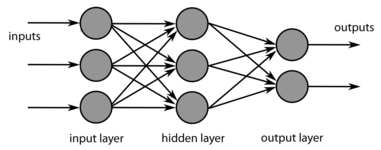
\includegraphics[scale=0.6]{figures/feedforwardnetworkillustration.png}
    \caption{Illustration of feed forward neural network. }
    \label{fig:feedforwardnetwork}
\end{figure}

The network can be described as having an \textit{input layer}, that takes the covariates, $\textbf{x}$. The \textit{hidden layer} makes a transformation, of the previous layer, that also implies that a hidden layer, can be followed by an arbitrary number of other hidden layers. Lastly and \textit{output layer} that maps the representation of the hidden layer into the desired output. For classification that might be a one-hot encoding of the classes, and for regression it might to a single real valued scalar.

As illustrated in figure \ref{fig:feedforwardnetwork}, each layers is broken down into smaller cells. The number of cells in each layer corresponds to the width of the layer. The wider the layer the more flexible representation the given layer is capable of doing. The hidden cells work as mentioned by creating a non-linear transformation of the input from last layer:

\begin{equation}
    z_i^{+} = g(\textbf{z}; \theta) = g(\textbf{w}^T \cdot \textbf{z} + b)
\end{equation}

The output of cell \textit{i} is the real valued scaler $z_i^+$. $g$ is the activation function that maps the input into the output. $\textbf{w}$ is the weights of dot product, $\textbf{z}$ is a vector of the outputs from the last layer, and $b$ is bias or the constant in the activation. In that sense the activation looks like a linear regression squashed through an activation function $g$. Multiple different activations functions has been proposed. Originally the logistic function was prefered, but in later years the rectified linear unit activation function has been popular \parencite{goodfellow_deep_2016}:

\begin{equation}
    \textbf{Rectified Linear Unit: }  \max \lcp 0, \textbf{w}^T \cdot \textbf{z} + b \rcp
\end{equation}

The neural network can in other words be considered a function $f$, that takes an input $\textbf{x}$ and maps it to some output $y$, parametrized by $\theta$, which is a collection of all the weights and biases associated with each individual cell.

\subsection{Stochastic Gradient Descent and Optimization}

The neural network is estimated (or trained) by using stochastic gradient descent. This is possible due to the fact, that the networks can be represented as set of nested functions, such that the chain rule can be applied. The loss function can in other words be differentiated with respect to the parameter vector $\theta$ as shown below:

\begin{equation}\label{eq:loss_function}
    \frac{\partial}{\partial\theta} \Loss (\textbf{X}, \textbf{Y}, \theta) = \frac{\partial}{\partial\theta} \lp \sum \ell_i \rp = \frac{\partial}{\partial\theta} \lp \sum \lp \hat{Y}_i  - Y_i \rp^2 \rp = \frac{\partial}{\partial\theta} \lp \sum \lp f^{\theta}(X_i)  - Y_i \rp^2 \rp
\end{equation}

In equation \eqref{eq:loss_function} the loss function $\Loss$ is assumed be be a mean squared error, in other words a regression problem. The optimization works by trying to minimize this loss with respect to the parameters $\theta$. In modern neural network architectures it's not unusual that such network has in around a million parameters, and furthermore the objective function of the optimization cannot be assumed to be convex. This implies that analytical solutions for solving deep neural networks is infeasible. Instead gradient descent is used for estimating the parameters of the network. So the objective function can be described as \parencite{goodfellow_deep_2016}:

\begin{equation}
    \theta \la \theta - \alpha \nabla_{\theta} \Loss(\textbf{X}, \textbf{Y}, \theta)
\end{equation}

So for each step in the algorithm the derivative with of the loss function with respect to the parameters can be calculated, and the parameters can be updated by taking a small step of size $\alpha$ in the direction in parameter space that reduces the loss. Stochastic gradient descent is the insight that in can computationally expensive to calculate the gradient for the entire data set in each step iteration of the algorithm. This is important for deep neural networks, since the training period of a large network, even on optimized hardware, can take a very long time, so any speed up for the training is important. 





\subsection{Historical overview}

\subsection{Theoretical considerations}




